\documentclass[aspectratio=169,11pt]{beamer}

% Shared style (ib-tutorials.sty at the repo root).
\makeatletter\def\input@path{{./}{../}}\makeatother
\usepackage{ib-tutorials}

\usepackage[utf8]{inputenc}
\usepackage{amsmath,amssymb}
\usepackage{booktabs}
\usepackage{array}
\newcolumntype{L}[1]{>{\raggedright\arraybackslash}p{#1}}
\usepackage{graphicx}
\graphicspath{{../pictures/4-ibfe/}{pictures/4-ibfe/}}
\usepackage{xcolor}
\usepackage{listings}
\usepackage{tikz}
\usetikzlibrary{arrows.meta,positioning,shapes.geometric,fit,calc,decorations.pathmorphing}
\usepackage{hyperref}

\newcommand{\sourcecredit}[1]{\vfill\begin{flushright}\tiny\textcolor{DarkGray}{#1}\end{flushright}}

\lstset{
  basicstyle=\ttfamily\scriptsize\color{BlackGray},
  keywordstyle=\color{NavyBlue}\bfseries,
  commentstyle=\color{DarkGray}\itshape,
  stringstyle=\color{OliveGreen},
  showstringspaces=false,
  columns=fullflexible,
  keepspaces=true,
  breaklines=true,
  breakindent=1em,
  frame=single,
  framerule=0.4pt,
  rulecolor=\color{LightGray},
  backgroundcolor=\color{LightGray!30},
  xleftmargin=0.25em,
  xrightmargin=0.25em
}
\lstdefinestyle{shell}{morecomment=[l]{\#}}
\lstdefinestyle{input}{morecomment=[l]{//}}
\lstdefinestyle{matlab}{morecomment=[l]{\%}}
\lstdefinestyle{python}{morecomment=[l]{\#}}
\lstdefinestyle{data}{}
\lstdefinestyle{tiny}{basicstyle=\ttfamily\tiny\color{BlackGray}}
\lstdefinestyle{inputtiny}{morecomment=[l]{//},basicstyle=\ttfamily\tiny\color{BlackGray}}
\lstdefinestyle{cpp}{language=C++,morecomment=[l]{//}}
\lstdefinestyle{cpptiny}{language=C++,morecomment=[l]{//},basicstyle=\ttfamily\tiny\color{BlackGray}}
\lstdefinestyle{cppmicro}{language=C++,morecomment=[l]{//},basicstyle=\ttfamily\fontsize{5.6}{6.6}\selectfont\color{BlackGray}}

\title[Walking through a main file]{Walking through an IBFE main file}
\subtitle{IBAMR's \code{IBFE/explicit/ex7}, a collapsible channel, read from the first \code{\#include} to \code{output\_data}: what each block does, which input keys it reads, what the libraries behind it are, how the 2020 version differs, and the sponge layer that the input never turns on}
\author[Miller]{Laura A. Miller}
\institute[UArizona]{Department of Mathematics, University of Arizona}
\date{Using IB Software \textbullet\ Part IV \textbullet\ Chapter 23}

\begin{document}

% 1
\begin{frame}[plain]
\maketutorialtitlepanel{%
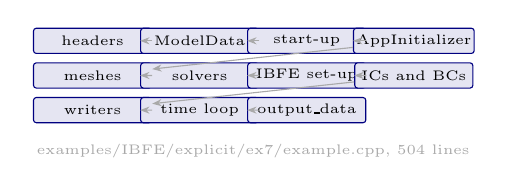
\begin{tikzpicture}[scale=0.8, every node/.style={font=\tiny}]
  \foreach \i/\t in {0/headers, 1/ModelData, 2/start-up, 3/AppInitializer, 4/meshes, 5/solvers, 6/IBFE set-up, 7/ICs and BCs, 8/writers, 9/time loop, 10/output\_data} {
    \node[draw=NavyBlue,fill=NavyBlue!10,rounded corners=1pt,minimum width=1.5cm,minimum height=0.32cm,inner sep=1pt] (b\i) at ({mod(\i,4)*1.7}, {-floor(\i/4)*0.55}) {\t};
  }
  \foreach \i [evaluate=\i as \j using int(\i+1)] in {0,...,9} { \draw[-{Stealth[length=1.2mm]},DarkGray] (b\i) -- (b\j); }
  \node[text=DarkGray] at (2.55,-1.75) {\code{examples/IBFE/explicit/ex7/example.cpp}, 504 lines};
\end{tikzpicture}}
\end{frame}

% 2
\begin{frame}{Learning goals}
\label{fr:goals}
\footnotesize By the end of this chapter you should be able to:
\begin{enumerate}
  \item name the blocks every IBAMR main file has, in order, and say what each one does and which input-file block it reads;
  \item read the C++ you meet there (namespaces, classes and their member functions, \code{Pointer<>}, headers, \code{static} globals, callbacks) well enough to follow any example, and find the rest in the documentation;
  \item explain IBAMR's \code{ex7}: a channel with a flexible segment in its upper wall held by an external pressure, three cases, and what the run produces;
  \item say what \code{IBTKInit}, \code{AppInitializer}, the solver objects, the gridding objects and the writers are, and what the time loop asks of them;
  \item tell the 2020 version of the file from today's and update one to the other;
  \item explain what the sponge layer does and why, in \code{ex7} as shipped, it does nothing.
\end{enumerate}
\begin{punchbox}
\footnotesize The 2020 lecture said: ``The approach I will use can be applied to understanding other IBAMR examples.'' That is the point: one file read closely, then the same map on every other.
\end{punchbox}
\end{frame}

% 3
\begin{frame}{Where this chapter comes from}
\label{fr:sources}
\scriptsize
\begin{itemize}
  \item \al{``Lecture 8-IBFE-Going through a main file'' (August 2020; 30 slides; \code{IBFE\_Lecture\_8}):} the IBAMR stack, a C++ primer (namespaces, classes, headers), then \code{ex7} block by block in nine code screenshots with one- or two-line notes (``Pick your Navier Stokes solver'', ``Write initial visit and exodus files'', ``Not totally sure what sponge layer does''). Its C++ slides quoted \code{tutorialspoint.com} and its stack slides IBAMR's README: both are rewritten here in this series' words; the screenshots are transcribed from the 0.19.0 file and the 2020 differences listed.
  \item \al{IBAMR 0.19.0, \code{examples/IBFE/explicit/ex7}:} \code{example.cpp} (504 lines), three inputs \code{input2d.caseC}, \code{caseS2}, \code{caseSP}; \code{ibtk/AppInitializer.cpp}, \code{IBTKInit.cpp}, \code{SpongeLayerForceFunction.cpp} for what the calls do.
  \item \al{The run:} \code{caseC} built against 0.19.0 with the six-line \code{CMakeLists.txt} of chapter 15 and run to $t = 2$ s on four cores; its figures and cost are on slides \ref{fr:run}--\ref{fr:see2}.
  \item \al{New here:} the order-of-blocks map; the input-key aliases \code{AppInitializer} accepts; the three cases compared; the sponge layer explained from its source, and the key-name mismatch that leaves it off; the 2020-to-now table; the recipe for reading any other example.
\end{itemize}
\end{frame}

% 4
\begin{frame}{The stack under a main file (1)}
\label{fr:stack}
\footnotesize
\setlength{\tabcolsep}{3pt}
\begin{tabular}{@{}L{0.12\textwidth}L{0.46\textwidth}L{0.38\textwidth}@{}}
\toprule
library & what it does in an IBFE program & where you meet it \\
\midrule
SAMRAI & the Cartesian grid, its levels and patches, the input database, restart files, timers & \code{Pointer<Database>}, \code{PatchHierarchy}, \code{CartesianGridGeometry}, \code{GriddingAlgorithm} \\
PETSc & linear solvers and the MPI start-up; \code{-ksp\_*} options & \code{petscsys.h}, \code{petsc\_options\_file} \\
libMesh & the finite element mesh, its systems and degrees of freedom, ExodusII output & \code{Mesh}, \code{MeshTools::Generation}, \code{EquationSystems}, \code{ExodusII\_IO} \\
hypre & the multigrid preconditioners behind the pressure and velocity solves & the input's \code{stokes\_solver\_db} (chapter 16) \\
IBTK & IBAMR's toolkit: \code{AppInitializer}, \code{IBTKInit}, muParser functions, \code{IBTK\_MPI} & \code{ibtk/*.h} \\
IBAMR & the IB methods and the fluid solvers & \code{IBFEMethod}, \code{IBExplicitHierarchyIntegrator}, \code{INSStaggeredHierarchyIntegrator} \\
\bottomrule
\end{tabular}

\medskip
The 2020 slide 2 listed these from IBAMR's README; the column on the right is what the list means when you read a main file.
\end{frame}

% 4b
\begin{frame}{The stack under a main file (2)}
\label{fr:stack2}
\footnotesize
\setlength{\tabcolsep}{3pt}
\begin{tabular}{@{}L{0.16\textwidth}L{0.46\textwidth}L{0.34\textwidth}@{}}
\toprule
library & what it does & where you meet it \\
\midrule
Boost & multi-dimensional arrays & \code{boost::multi\_array} (chapter 22's post-processing) \\
Eigen & small dense linear algebra & inside IBAMR; \code{app\_namespaces.h} brings it in \\
HDF5 & binary files for restarts and state dumps & \code{HDFDatabase} (slide \ref{fr:outputdata}) \\
muParser & the expressions in the input (\code{"U0*tanh(2*t)"}) & \code{muParserCartGridFunction}, \code{muParserRobinBcCoefs} \\
Silo & the point method's Lagrangian output (Part III) & \code{lag\_data.visit} \\
MPI & the processes; \code{mpirun -np 4} & \code{IBTK\_MPI::getRank()}, \code{sumReduction} \\
VisIt & reads what the writers write & \code{dumps.visit}, \code{*.ex2} \\
\bottomrule
\end{tabular}

\medskip
\begin{itemize}
  \item ``IBAMR requires a number of third-party libraries. Sample build instructions are provided for a typical Linux installation and macOS. We offer experimental support the use of Windows 10 through the Windows Subsystem for Linux (WSL)'' (2020, slide 3, from the README). autoibamr builds the whole stack (chapter 3); this series' WSL runs are the ``experimental'' route, and it works.
  \item A main file touches each library in one or two lines; the rest is inside IBAMR.
\end{itemize}
\end{frame}

% 5
\begin{frame}[fragile]{Reading the C++ (1): namespaces and classes}
\label{fr:cpp}
\footnotesize
\begin{lstlisting}[style=cpptiny]
#include <ibamr/IBFEMethod.h>            // the class's declaration
#include <ibamr/app_namespaces.h>        // "using namespace" for IBAMR, IBTK, SAMRAI, libMesh, std, ...
Pointer<IBFEMethod> ib_method_ops =      // a reference-counted pointer to an object
    new IBFEMethod("IBFEMethod", input_db->getDatabase("IBFEMethod"), meshes, max_levels);
ib_method_ops->registerPK1StressFunction(data, 0);   // a member function, called through the pointer
IBFEMethod::PK1StressFcnData data(PK1_fcn);          // a type nested in the class; built from a function
static double kappa_s = 1.0e6;           // a file-wide variable the callbacks can see
namespace ModelData { ... }              // a named scope for the model's functions and constants
\end{lstlisting}
\begin{itemize}
  \item \al{A namespace is a named scope.} \code{IBAMR::IBFEMethod} is the class \code{IBFEMethod} in the namespace \code{IBAMR}; two libraries can both have a \code{Point} without clashing. \code{app\_namespaces.h} writes the \code{using namespace} lines for you, so the examples say \code{Pointer}, \code{Mesh}, \code{VectorValue} without prefixes. It must be included only in a main file, never in a header: a header that did it would force the choice on every file that includes it.
  \item \al{A class bundles data with the functions that act on it.} \code{ib\_method\_ops} is an object; \code{->} calls one of its member functions; \code{IBFEMethod::PK1StressFcnData} is a small class that lives inside \code{IBFEMethod}. The 2020 slides 5--6 explained both with a tutorial's words (``two persons with the same name, Zara''); for IBAMR the two examples above are the whole of it.
\end{itemize}
\end{frame}

% 5b
\begin{frame}{Reading the C++ (2): pointers, headers, statics, callbacks}
\label{fr:cpp2}
\footnotesize
\begin{itemize}
  \item \al{\code{Pointer<T>}} is SAMRAI's smart pointer: it counts references and deletes the object when the last one goes; \code{new} creates the object; \code{setNull()} drops it. libMesh and the standard library use \code{std::unique\_ptr} for the same job; the examples mix the two, one per library.
  \item \al{A header file} (\code{.h}) declares what a library offers; \code{\#include} pastes it in. Every class you use needs its header; the compiler's ``was not declared in this scope'' means one is missing. ``Including a header file is equal to copying the content of the header file'' (2020, slide 9).
  \item \al{\code{static} at file scope} makes a variable private to this file; the model's constants are declared so, set from the input in \code{main}, and read by the callbacks, which cannot take extra arguments.
  \item \al{A callback} is a function you write and hand to IBAMR, which calls it when it needs a stress or a force (chapter 19): its signature is fixed by IBAMR, and \code{/*X*/} in the signature marks an argument the function does not use.
  \item \al{Where to look:} \url{https://ibamr.github.io/docs}, the search box, and the ``Classes'' tab: a class's page is its header made readable, with every member function and what it takes. ``In general, I perform searches here to learn more about various functions and classes'' (2020, slide 4), and ``at some point, I recommend really learning C++.''
\end{itemize}
\end{frame}

% 6
\begin{frame}{What \code{ex7} is: a collapsible channel}
\label{fr:ex7}
\footnotesize
\begin{center}
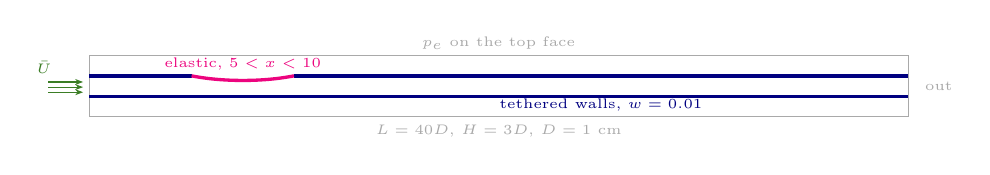
\begin{tikzpicture}[scale=0.26, every node/.style={font=\tiny}]
  \draw[DarkGray] (0,0) rectangle (40,3);
  \draw[NavyBlue,very thick] (0,1) -- (40,1);
  \draw[NavyBlue,very thick] (0,2) -- (5,2); \draw[NavyBlue,very thick] (10,2) -- (40,2);
  \draw[RubineRed,very thick] (5,2) .. controls (6.5,1.7) and (8.5,1.7) .. (10,2);
  \foreach \y in {1.2,1.45,1.7} \draw[-{Stealth[length=1mm]},OliveGreen] (-2,\y) -- (-0.3,\y);
  \node[text=OliveGreen] at (-2.2,2.4) {$\bar U$};
  \node[text=RubineRed] at (7.5,2.6) {elastic, $5 < x < 10$};
  \node[text=NavyBlue] at (25,0.55) {tethered walls, $w = 0.01$};
  \node[text=DarkGray] at (20,3.6) {$p_e$ on the top face};
  \node[text=DarkGray] at (41.5,1.5) {out};
  \node[text=DarkGray] at (20,-0.7) {$L = 40D$, $H = 3D$, $D = 1$ cm};
\end{tikzpicture}
\end{center}
\begin{itemize}
  \item Two thin walls, one element thick, built in the program with \code{build\_square}: the lower at $y = D$, the upper at $y = 2D$, in a box $40D\times3D$. The channel is the slot between them; the fluid above and below the walls is ``outside''.
  \item The lower wall and the upper wall's rigid parts are held by tethers; the segment $5 < x < 10$ of the upper wall is elastic (St.\ Venant--Kirchhoff, $E = 4.8\times10^6$ dyn/cm$^2$, $\nu = 0.45$) and untethered.
  \item A parabolic inflow of mean $\bar U$ enters at $x = 0$ between the walls, ramped up over $\tau = 1$ s; the outflow at $x = 40$ is traction-free; the top face carries the external pressure $p_e$ as a normal stress, so the fluid above the upper wall presses on the elastic segment from outside while the channel's own pressure presses from inside. Which way the segment goes depends on which is larger (slide \ref{fr:see2}).
  \item The lengths ($5D$ rigid, $5D$ flexible, $30D$ rigid) and the external pressure are the collapsible-channel problem of Luo and Pedley (1996), where a flexible segment buckles and oscillates as the flow and $p_e$ compete; here the segment is a thin elastic wall rather than a membrane under tension.
\end{itemize}
\end{frame}

% 6b
\begin{frame}{\code{ex7} (2): the three cases}
\label{fr:cases}
\footnotesize
\begin{center}
\begin{tabular}{@{}L{0.22\textwidth}lll@{}}
\toprule
& \code{caseC} & \code{caseS2} & \code{caseSP} \\
\midrule
$\bar U$ (cm/s) & $5$ & $2$ & $0.771$ \\
$\mathrm{Re} = \rho\bar U D/\mu$ & $500$ & $200$ & $77$ \\
$p_e$ (dyn/cm$^2$) & $48.75$ & $8.60$ & $17.55$ \\
$E$ (dyn/cm$^2$) & $4.79\times10^6$ & $1.76\times10^5$ & $7.18\times10^5$ \\
inflow & velocity & velocity & pressure $p_u = 4.5$ \\
\code{END\_TIME} & $1000\,\mathrm{DT}$ & $100$ s & $100$ s \\
\bottomrule
\end{tabular}
\end{center}
\begin{itemize}
  \item \code{caseC}'s \code{END\_TIME} is $1000$ steps, $0.02$ s: a check that it runs. The two others run $100$ s, five million steps; slide \ref{fr:see} runs \code{caseC} to $2$ s.
  \item \code{caseSP} drives the flow by a pressure difference instead of a velocity: the inflow face's \code{acoef} is $0$ and \code{bcoef} $1$ inside the channel with $g = -p_u$ (a traction), and $\bar U$ is only used to size the time step.
  \item Water: $\rho = 1$, $\mu = 0.01$ in cgs; $\mathrm{DX} = 3/96 = 0.031$ cm on four levels at ratio $2$; $\mathrm{DT} = 0.0125\,\mathrm{DX}/U_{\max} = 2\times10^{-5}$ s with $U_{\max} = 4\bar U$.
  \item $\mu_s = E/(2(1+\nu))$ and $\lambda_s = E\nu/((1+\nu)(1-2\nu))$ as in chapter 22; $\nu = 0.45$ makes the wall nearly incompressible, $\lambda_s = 9\mu_s$.
\end{itemize}
\end{frame}

% 7
\begin{frame}{The map (1): what every IBAMR main file does, in order}
\label{fr:map}
\scriptsize
\setlength{\tabcolsep}{3pt}
\begin{tabular}{@{}L{0.03\textwidth}L{0.19\textwidth}L{0.44\textwidth}L{0.28\textwidth}@{}}
\toprule
& block & what it does & reads from the input \\
\midrule
1 & headers & the libraries' declarations; \code{app\_namespaces.h} last & \\
2 & \code{ModelData} & the model's constants and callbacks: stresses, forces, mappings & (set in \code{main}) \\
3 & prototypes & \code{output\_data}'s declaration, so \code{main} can call it & \\
4 & start-up & \code{IBTKInit}: MPI, PETSc, SAMRAI, libMesh up and, at the end, down & \code{petsc\_options\_file} \\
5 & \code{AppInitializer} & the command line, the input file, the log, restart, the writers' settings & \code{Main} \\
6 & meshes & build or read the bodies; the vector of parts & \code{DX}, \code{MFAC}, \code{ELEM\_TYPE}, \code{MESH\_FILENAME} \\
7 & solvers & the fluid solver, \code{IBFEMethod}, the IB time integrator & \code{Main.solver\_type}, the three solver blocks \\
8 & grid objects & geometry, hierarchy, tagging, box generation, load balancing, gridding & \code{CartesianGeometry}, \code{GriddingAlgorithm}, \code{StandardTagAndInitialize}, \code{LoadBalancer} \\
9 & IBFE set-up & register the callbacks per part; \code{initializeFEEquationSystems()} & \code{IBFEMethod} (through the constructor) \\
\bottomrule
\end{tabular}
\end{frame}

% 7b
\begin{frame}{The map (2)}
\label{fr:map2}
\scriptsize
\setlength{\tabcolsep}{3pt}
\begin{tabular}{@{}L{0.03\textwidth}L{0.19\textwidth}L{0.44\textwidth}L{0.28\textwidth}@{}}
\toprule
& block & what it does & reads from the input \\
\midrule
10 & ICs and BCs & muParser functions for the initial velocity and pressure; Robin coefficients per face & \code{VelocityInitialConditions}, \code{PressureInitialConditions}, \code{VelocityBcCoefs\_d} \\
11 & body force & an Eulerian force on the fluid (here the sponge layer) & \code{ForcingFunction} or \code{SpongeLayerForceFunction} \\
12 & writers & VisIt for the grid, one ExodusII per part; append on restart & \code{viz\_*}, \code{exodus\_filename} \\
13 & initialize & \code{initializeFEData()}, \code{initializePatchHierarchy()}; drop the initializer; log the input & \\
14 & initial dump & frame $0$ & \\
15 & time loop & step, then at intervals: viz, restart, timers, post-processing & the intervals \\
16 & clean-up & delete the boundary objects; the braces end everything else & \\
17 & \code{output\_data} & whatever you measure (chapter 11, chapter 22) & \code{data\_*} \\
\bottomrule
\end{tabular}

\medskip
\begin{itemize}
  \item The course's \code{main.C} files (chapters 17--22) have the same seventeen blocks; IBAMR's IB examples (chapter 15) replace blocks 6 and 9 by the point-method's \code{IBStandardInitializer} and \code{IBMethod}.
  \item Blocks 4, 5, 7, 8, 12, 13 and 15 are copied unchanged from example to example; 2, 6, 9, 10, 11 and 17 are where a model lives.
\end{itemize}
\end{frame}

% 8
\begin{frame}[fragile]{Block 1: the headers}
\label{fr:headers}
\begin{columns}[T]
\column{0.5\textwidth}
\begin{lstlisting}[style=cpptiny]
// Config files
#include <SAMRAI_config.h>
// Headers for basic PETSc functions
#include <petscsys.h>
// Headers for basic SAMRAI objects
#include <BergerRigoutsos.h>
#include <CartesianGridGeometry.h>
#include <LoadBalancer.h>
#include <StandardTagAndInitialize.h>
// Headers for basic libMesh objects
#include <libmesh/boundary_info.h>
#include <libmesh/equation_systems.h>
#include <libmesh/exodusII_io.h>
#include <libmesh/mesh.h>
#include <libmesh/mesh_generation.h>
\end{lstlisting}
\column{0.5\textwidth}
\begin{lstlisting}[style=cpptiny]
// Headers for application-specific algorithm/data structure objects
#include <ibamr/IBExplicitHierarchyIntegrator.h>
#include <ibamr/IBFEMethod.h>
#include <ibamr/INSCollocatedHierarchyIntegrator.h>
#include <ibamr/INSStaggeredHierarchyIntegrator.h>
#include <ibamr/SpongeLayerForceFunction.h>
#include <ibtk/AppInitializer.h>
#include <ibtk/IBTKInit.h>
#include <ibtk/IBTK_MPI.h>
#include <ibtk/libmesh_utilities.h>
#include <ibtk/muParserCartGridFunction.h>
#include <ibtk/muParserRobinBcCoefs.h>
// Set up application namespace declarations
#include <ibamr/app_namespaces.h>
\end{lstlisting}
\end{columns}
\scriptsize
\begin{itemize}
  \item Five groups: SAMRAI's configuration and its four grid classes; PETSc's base header; libMesh's mesh, generator, systems and ExodusII writer; IBAMR's two fluid solvers, the IB integrator, \code{IBFEMethod} and the sponge layer; IBTK's start-up, initializer, MPI wrapper, libMesh helpers and the two muParser classes. Then the namespaces, last.
  \item The 2020 file began with \code{\#include <IBAMR\_config.h>} and \code{<IBTK\_config.h>} and had no \code{IBTKInit.h} or \code{IBTK\_MPI.h}: the headers are the quickest way to date a file (chapter 17).
  \item \code{mesh\_generation.h} is here because \code{ex7} builds its walls in the program; a program that reads a mesh file needs \code{mesh.h} only. \code{SpongeLayerForceFunction.h} is the 2020 ``example header file'' (slide 10): ``provides forcing at physical boundaries that weakly imposes homogeneous Dirichlet boundary conditions'', slide \ref{fr:sponge}.
\end{itemize}
\end{frame}

% 9
\begin{frame}[fragile]{Block 2: \code{ModelData}, the model in callbacks}
\label{fr:model}
\begin{lstlisting}[style=cpptiny]
namespace ModelData
{
// Stress tensor function.
static double mu_s, lambda_s;
void upper_PK1_stress_function(TensorValue<double>& PP, const TensorValue<double>& FF, const libMesh::Point& /*X*/, const libMesh::Point& s,
                               Elem* const /*elem*/, const vector<const vector<double>*>& /*var_data*/,
                               const vector<const vector<VectorValue<double>>*>& /*grad_var_data*/, double /*time*/, void* /*ctx*/)
{
    if (s(0) > 5.0 && s(0) < 10.0)
    {
        static const TensorValue<double> II(1.0, 0.0, 0.0, 0.0, 1.0, 0.0, 0.0, 0.0, 1.0);
        const TensorValue<double> CC = FF.transpose() * FF;
        const TensorValue<double> EE = 0.5 * (CC - II);
        const TensorValue<double> SS = lambda_s * EE.tr() * II + 2.0 * mu_s * EE;
        PP = FF * SS;
    }
    else { PP.zero(); }
    return;
} // upper_PK1_stress_function
// Tether (penalty) force functions for lower and upper blocks.
static double kappa_s = 1.0e6;
void lower_tether_force_function(VectorValue<double>& F, ..., const libMesh::Point& X, const libMesh::Point& s, ...)
{   F = kappa_s * (s - X);  return; }
void upper_tether_force_function(VectorValue<double>& F, ..., const libMesh::Point& X, const libMesh::Point& s, ...)
{   if (s(0) > 5.0 && s(0) < 10.0) { F.zero(); } else { F = kappa_s * (s - X); }  return; }
} // namespace ModelData
using namespace ModelData;
\end{lstlisting}
\end{frame}

% 9b
\begin{frame}{Block 2 (2): what the callbacks say}
\label{fr:model2}
\footnotesize
\begin{itemize}
  \item The St.\ Venant--Kirchhoff stress of chapter 19 (slide 13) on the elastic segment: $\mathbb{C} = \mathbb{F}^T\mathbb{F}$, $\mathbb{E} = \tfrac12(\mathbb{C} - \mathbb{I})$, $\mathbb{S} = \lambda_s\,\mathrm{tr}\,\mathbb{E}\,\mathbb{I} + 2\mu_s\mathbb{E}$, $\mathbb{P} = \mathbb{F}\mathbb{S}$; and \emph{zero} elsewhere. The rigid parts have no stiffness of their own, only the tether. \code{II} is written with nine entries, a 3D identity; in 2D libMesh's \code{TensorValue} ignores the third row and column.
  \item The upper tether is the complement: zero on the segment, $\kappa_s(\mathbf{s} - \mathbf{X})$ elsewhere. The lower wall is tethered everywhere and has no stress function at all: a part without stiffness (chapter 21), which is what a rigid wall held by a stiff tether should be.
  \item The segment is attached to the rigid parts only through the shared nodes at $x = 5$ and $x = 10$; the elastic stress there pulls on nodes the tether holds, so the segment is clamped.
  \item $\mu_s$, $\lambda_s$ and $\kappa_s$ are \code{static} and set from the input in \code{main} (2020, slide 18: ``kappa\_s = target force stiffness''); the \code{1.0e6} is a default that the input overrides with $2.5\,\mathrm{DX}/\mathrm{DT}^2 = 2\times10^9$.
  \item \code{using namespace ModelData;} after the namespace lets \code{main} write \code{kappa\_s} without the prefix; the course's files do the same.
\end{itemize}
\end{frame}

% 10
\begin{frame}[fragile]{Block 4: the start-up, then and now}
\label{fr:startup}
\footnotesize
\begin{columns}[T]
\column{0.5\textwidth}
2020 (slide 12, ``Main function''):
\begin{lstlisting}[style=cpptiny]
int
main(int argc, char* argv[])
{
    // Initialize libMesh, PETSc, MPI, and SAMRAI.
    LibMeshInit init(argc, argv);
    SAMRAI_MPI::setCommunicator(PETSC_COMM_WORLD);
    SAMRAI_MPI::setCallAbortInSerialInsteadOfExit();
    SAMRAIManager::startup();
    { // cleanup dynamically allocated objects prior to shutdown
        ...
    }
    SAMRAIManager::shutdown();
    return 0;
}
\end{lstlisting}
\column{0.48\textwidth}
0.19.0:
\begin{lstlisting}[style=cpptiny]
int
main(int argc, char* argv[])
{
    // Initialize IBAMR and libraries. Deinitialization is handled by this object as well.
    IBTKInit ibtk_init(argc, argv, MPI_COMM_WORLD);
    const LibMeshInit& init = ibtk_init.getLibMeshInit();
    { // cleanup dynamically allocated objects prior to shutdown
        ...
    } // cleanup dynamically allocated objects prior to shutdown
} // main
\end{lstlisting}
\end{columns}
\begin{itemize}
  \item \code{IBTKInit}'s constructor calls \code{PetscInitialize}, sets SAMRAI's and IBTK's communicators, raises SAMRAI's patch-data limit to $2048$, starts \code{SAMRAIManager} and libMesh; its destructor shuts them down in the right order. ``Attempts to create a second IBTKInit object will result in a run time error.''
  \item \code{init} is what \code{Mesh} needs (\code{Mesh mesh(init.comm(), NDIM)}); the 2020 \code{Mesh mesh(NDIM)} is the old libMesh signature (chapter 17).
  \item The inner braces matter: every object made inside them is destroyed before the libraries shut down. Objects created outside them are destroyed after, and crash.
\end{itemize}
\end{frame}

% 11
\begin{frame}[fragile]{Block 5: \code{AppInitializer} (1): the command line, the log, the writers}
\label{fr:appinit}
\begin{lstlisting}[style=cpptiny]
// Parse command line options, set some standard options from the input
// file, initialize the restart database (if this is a restarted run),
// and enable file logging.
Pointer<AppInitializer> app_initializer = new AppInitializer(argc, argv, "IB.log");
Pointer<Database> input_db = app_initializer->getInputDatabase();
// Get various standard options set in the input file.
const bool dump_viz_data = app_initializer->dumpVizData();
const int viz_dump_interval = app_initializer->getVizDumpInterval();
const bool uses_visit = dump_viz_data && app_initializer->getVisItDataWriter();
#ifdef LIBMESH_HAVE_EXODUS_API
const bool uses_exodus = dump_viz_data && !app_initializer->getExodusIIFilename().empty();
#else
const bool uses_exodus = false;
if (!app_initializer->getExodusIIFilename().empty())
{
    plog << "WARNING: libMesh was compiled without Exodus support, so no "
         << "Exodus output will be written in this program.\n";
}
#endif
const string lower_exodus_filename = app_initializer->getExodusIIFilename("lower");
const string upper_exodus_filename = app_initializer->getExodusIIFilename("upper");
\end{lstlisting}
\scriptsize
\begin{itemize}
  \item \code{argv}: the input file, and for a restart the restart directory and number (\code{main2d input2d restart\_IB2d 5000}); \code{"IB.log"} is the default log name, which \code{log\_file\_name} in \code{Main} overrides.
  \item \code{\#ifdef LIBMESH\_HAVE\_EXODUS\_API}: a libMesh built without ExodusII support compiles the program without the writer; autoibamr builds it with. \code{getExodusIIFilename("lower")}: chapter 21's prefix rule, \code{loweroutput.ex2}.
\end{itemize}
\end{frame}

% 11b
\begin{frame}[fragile]{Block 5 (2): restart, post-processing and timers}
\label{fr:appinit2}
\begin{lstlisting}[style=cpptiny]
const bool dump_restart_data = app_initializer->dumpRestartData();
const int restart_dump_interval = app_initializer->getRestartDumpInterval();
const string restart_dump_dirname = app_initializer->getRestartDumpDirectory();
const string restart_read_dirname = app_initializer->getRestartReadDirectory();
const int restart_restore_num = app_initializer->getRestartRestoreNumber();
const bool dump_postproc_data = app_initializer->dumpPostProcessingData();
const int postproc_data_dump_interval = app_initializer->getPostProcessingDataDumpInterval();
const string postproc_data_dump_dirname = app_initializer->getPostProcessingDataDumpDirectory();
if (dump_postproc_data && (postproc_data_dump_interval > 0) && !postproc_data_dump_dirname.empty())
{
    Utilities::recursiveMkdir(postproc_data_dump_dirname);
}
const bool dump_timer_data = app_initializer->dumpTimerData();
const int timer_dump_interval = app_initializer->getTimerDumpInterval();
\end{lstlisting}
\scriptsize
\begin{itemize}
  \item \code{getInputDatabase()} is the whole input file as a tree of databases; \code{getComponentDatabase("X")} is one block of it, handed to the object that reads it.
  \item ``Determine intervals for writing restart files and post processing and writing data'' (2020, slide 14). \code{dumpVizData()} is true when the viz interval is positive; the same pattern for restart, post-processing (``data'') and timers; \code{dumpRestartData} ``return[s] a boolean value indicating whether to write restart data'' (slide 15, from the documentation).
  \item \code{recursiveMkdir} makes the data folder here; the viz and restart folders are made by their writers. The log collects \code{plog} from every process if \code{log\_all\_nodes = TRUE}, else rank $0$'s.
  \item The restart read directory and number come from the command line, not the input, so the same input serves the fresh run and every restart of it.
\end{itemize}
\end{frame}

% 11c
\begin{frame}{Block 5 (3): the \code{Main} block's keys and their aliases}
\label{fr:mainkeys}
\scriptsize
``getRestartDumpInterval \ldots can be defined in the input file as restart\_interval, restart\_dump\_interval, or restart\_write\_interval'' (2020, slide 15). From \code{AppInitializer.cpp}, the whole list:
\begin{center}
\setlength{\tabcolsep}{3pt}
\begin{tabular}{@{}L{0.2\textwidth}L{0.46\textwidth}L{0.28\textwidth}@{}}
\toprule
setting & accepted keys (first found wins) & default \\
\midrule
log file & \code{log\_file\_name}, \code{log\_all\_nodes} & the constructor's name; rank $0$ only \\
viz interval & \code{viz\_interval}, \code{viz\_dump\_interval}, \code{viz\_write\_interval} & $0$: no output \\
viz folder & \code{viz\_dirname}, \code{viz\_dump\_dirname}, \code{viz\_write\_dirname} & \\
viz writers & \code{viz\_writer}, \code{viz\_writers}: \code{"VisIt"}, \code{"ExodusII"}, \code{"Silo"}, \code{"GMV"} & \\
VisIt files & \code{visit\_number\_procs\_per\_file} & $1$ \\
ExodusII name & \code{exodus\_filename} & \code{output.ex2} \\
restart interval, folder & \code{restart\_interval} / \code{\_dump\_} / \code{\_write\_}; \code{restart\_dirname} / \code{\_dump\_} / \code{\_write\_} & $0$ \\
data (post-processing) & \code{data\_interval} / \code{\_dump\_} / \code{\_write\_}; \code{data\_dirname} / \ldots & $0$ \\
timers & \code{timer\_interval} / \code{\_dump\_} / \code{\_write\_} & $0$ \\
PETSc options & \code{petsc\_options\_file} (top level, not in \code{Main}) & \\
\bottomrule
\end{tabular}
\end{center}
\begin{itemize}
  \item The examples use the \code{\_dump\_} spelling; course inputs mix them, and all three work. A misspelt key is silently ignored, which is how an interval ends up at its default $0$ and a run writes nothing.
  \item \code{viz\_dump\_interval = int(320.0/CFL\_MAX)} in \code{ex7} is $3200$ steps, $0.0625$ s: the input language does arithmetic, and a key can be defined from an earlier one.
\end{itemize}
\end{frame}

% 12
\begin{frame}[fragile]{Block 6: the meshes, built in the program}
\label{fr:meshes}
\begin{lstlisting}[style=cpptiny]
// Create a simple FE mesh.
const double dx = input_db->getDouble("DX");
const double ds = input_db->getDouble("MFAC") * dx;
const double D = 1.0;      // channel height (cm)
const double L = 40.0 * D; // channel length (cm)
const double w = 0.01 * D; // wall thickness (cm)
string elem_type = input_db->getString("ELEM_TYPE");
Mesh lower_mesh(init.comm(), NDIM);
MeshTools::Generation::build_square(lower_mesh, static_cast<int>(ceil(L / ds)), static_cast<int>(ceil(w / ds)),
                                    0.0, L, D - 0.5 * w, D + 0.5 * w, Utility::string_to_enum<ElemType>(elem_type));
lower_mesh.prepare_for_use();
Mesh upper_mesh(init.comm(), NDIM);
MeshTools::Generation::build_square(upper_mesh, static_cast<int>(ceil(L / ds)), static_cast<int>(ceil(w / ds)),
                                    0.0, L, 2.0 * D - 0.5 * w, 2.0 * D + 0.5 * w, Utility::string_to_enum<ElemType>(elem_type));
upper_mesh.prepare_for_use();
vector<MeshBase*> meshes(2);
meshes[0] = &lower_mesh;
meshes[1] = &upper_mesh;
mu_s = input_db->getDouble("MU_S");
lambda_s = input_db->getDouble("LAMBDA_S");
kappa_s = input_db->getDouble("KAPPA_S");
\end{lstlisting}
\footnotesize
\code{build\_square(mesh, nx, ny, xmin, xmax, ymin, ymax, type, gauss\_lobatto\_grid)} (the 2020 slide 17's table): a rectangle of \code{nx} by \code{ny} elements of \code{type}. ``These immersed boundaries are geometrically relatively simple, so libmesh is used to make the meshes.''
\end{frame}

% 12b
\begin{frame}{Block 6 (2): what the numbers come to}
\label{fr:meshes2}
\footnotesize
\begin{itemize}
  \item \code{ds = MFAC * DX} is the element size: with \code{MFAC = 1} and $\mathrm{DX} = 0.031$, \code{nx = ceil(40/0.031) = 1280} and \code{ny = ceil(0.01/0.031) = 1}: each wall is $1280$ \code{QUAD4} elements, one element thick, and $0.01$ cm thin, a third of a grid cell. This is the case where \code{MFAC} matters (chapter 18): the program sizes the mesh from the grid, and a finer grid gives a finer wall.
  \item The walls are thinner than a cell, so the kernel smears each into a band about four cells wide; the channel the fluid sees is $1$ cm high with soft edges. \code{IB\_point\_density = 3} puts three interaction points per cell along each wall element, enough that no fluid leaks between them (chapter 17).
  \item \code{prepare\_for\_use()} after building or reading; \code{init.comm()} is the communicator from the start-up.
  \item The vector of parts and their order (chapter 21): lower is part $0$, upper part $1$.
  \item The material constants are read here, after the \code{ModelData} statics exist and before any callback runs. \code{KAPPA\_S = 2.5e1*DX/(DT\^{}2)} in the input: $2\times10^9$, the stiffness scaled with the time step that chapter 19 (slide 26) discussed: the stiffest tether the explicit step allows.
\end{itemize}
\end{frame}

% 13
\begin{frame}[fragile]{Block 7: the solvers}
\label{fr:solvers}
\begin{lstlisting}[style=cpptiny]
// Create major algorithm and data objects that comprise the
// application.  These objects are configured from the input database
// and, if this is a restarted run, from the restart database.
Pointer<INSHierarchyIntegrator> navier_stokes_integrator;
const string solver_type = app_initializer->getComponentDatabase("Main")->getString("solver_type");
if (solver_type == "STAGGERED")
{
    navier_stokes_integrator = new INSStaggeredHierarchyIntegrator(
        "INSStaggeredHierarchyIntegrator", app_initializer->getComponentDatabase("INSStaggeredHierarchyIntegrator"));
}
else if (solver_type == "COLLOCATED")
{
    navier_stokes_integrator = new INSCollocatedHierarchyIntegrator(
        "INSCollocatedHierarchyIntegrator", app_initializer->getComponentDatabase("INSCollocatedHierarchyIntegrator"));
}
else
{
    TBOX_ERROR("Unsupported solver type: " << solver_type << "\n" << "Valid options are: COLLOCATED, STAGGERED");
}
Pointer<IBFEMethod> ib_method_ops =
    new IBFEMethod("IBFEMethod", app_initializer->getComponentDatabase("IBFEMethod"), meshes,
                   app_initializer->getComponentDatabase("GriddingAlgorithm")->getInteger("max_levels"),
                   /*register_for_restart*/ true, restart_read_dirname, restart_restore_num);
Pointer<IBHierarchyIntegrator> time_integrator =
    new IBExplicitHierarchyIntegrator("IBHierarchyIntegrator", app_initializer->getComponentDatabase("IBHierarchyIntegrator"),
                                      ib_method_ops, navier_stokes_integrator);
\end{lstlisting}
\end{frame}

% 13b
\begin{frame}{Block 7 (2): what the three objects are}
\label{fr:solvers2}
\footnotesize
\begin{itemize}
  \item ``Pick your Navier Stokes solver'' (2020, slide 19): \code{Main.solver\_type} chooses the staggered-grid solver (the one to use; chapter 6) or the collocated projection solver; each reads its own block, and both blocks are in every input so that the switch works. ``Class INSStaggeredHierarchyIntegrator provides a staggered-grid solver for the incompressible Navier-Stokes equations on an AMR grid hierarchy'' (slide 20, from the documentation).
  \item \code{INSHierarchyIntegrator} is the base class both share: the rest of the program talks to the base and does not care which it got. ``Class IBFEMethod is an implementation of the abstract base class IBStrategy'' (slide 21) in the same way: \code{IBMethod} (points), \code{IBFEMethod} (elements) and \code{ConstraintIBMethod} (chapter 14) all fit the same \code{IBExplicitHierarchyIntegrator}.
  \item \code{IBFEMethod}'s arguments: its block, the parts, \code{max\_levels} from the gridding block (so that the two agree), and the restart settings. \code{register\_for\_restart = true} saves its finite element data with the restart files.
  \item \code{IBExplicitHierarchyIntegrator} owns the time step: it asks the fluid solver and the IB object in turn (chapter 5's loop). Its block has \code{start\_time}, \code{end\_time}, \code{dt\_max}, \code{num\_cycles}, \code{regrid\_cfl\_interval}, \code{error\_on\_dt\_change}.
  \item \code{TBOX\_ERROR} prints and aborts on every process: the way IBAMR reports a bad input.
\end{itemize}
\end{frame}

% 14
\begin{frame}[fragile]{Block 8: the grid objects}
\label{fr:grid}
\begin{lstlisting}[style=cpptiny]
Pointer<CartesianGridGeometry<NDIM>> grid_geometry = new CartesianGridGeometry<NDIM>(
    "CartesianGeometry", app_initializer->getComponentDatabase("CartesianGeometry"));
Pointer<PatchHierarchy<NDIM>> patch_hierarchy = new PatchHierarchy<NDIM>("PatchHierarchy", grid_geometry);
Pointer<StandardTagAndInitialize<NDIM>> error_detector =
    new StandardTagAndInitialize<NDIM>("StandardTagAndInitialize", time_integrator,
                                       app_initializer->getComponentDatabase("StandardTagAndInitialize"));
Pointer<BergerRigoutsos<NDIM>> box_generator = new BergerRigoutsos<NDIM>();
Pointer<LoadBalancer<NDIM>> load_balancer =
    new LoadBalancer<NDIM>("LoadBalancer", app_initializer->getComponentDatabase("LoadBalancer"));
Pointer<GriddingAlgorithm<NDIM>> gridding_algorithm =
    new GriddingAlgorithm<NDIM>("GriddingAlgorithm", app_initializer->getComponentDatabase("GriddingAlgorithm"),
                                error_detector, box_generator, load_balancer);
\end{lstlisting}
\scriptsize
Six SAMRAI objects, always these six, in this order:
\begin{itemize}
  \item \al{\code{CartesianGridGeometry}:} the box, its level-0 cells, which directions are periodic (\code{domain\_boxes}, \code{x\_lo}, \code{x\_up}, \code{periodic\_dimension}; chapter 7). \al{\code{PatchHierarchy}:} the levels and their patches; empty until \code{initializePatchHierarchy}.
  \item \al{\code{StandardTagAndInitialize}:} asks the time integrator which cells to refine (\code{tagging\_method = "GRADIENT\_DETECTOR"}: the integrator's own rule, vorticity thresholds and Lagrangian points). \al{\code{BergerRigoutsos}:} turns tagged cells into rectangular patches. \al{\code{LoadBalancer}:} hands the patches to processes (\code{bin\_pack\_method = "SPATIAL"}).
  \item \al{\code{GriddingAlgorithm}:} runs the three above: \code{max\_levels}, \code{ratio\_to\_coarser}, patch sizes, \code{efficiency\_tolerance}, \code{combine\_efficiency} (chapter 22, slide 20). \code{NDIM} is set when the program is compiled for 2D or 3D (\code{IBAMR::IBAMR2d} against \code{IBAMR3d}); the same source builds both.
\end{itemize}
\end{frame}

% 15
\begin{frame}[fragile]{Block 9: configure the IBFE solver}
\label{fr:ibfe}
\begin{lstlisting}[style=cpptiny]
// Configure the IBFE solver.
IBFEMethod::LagBodyForceFcnData lower_tether_force_data(lower_tether_force_function);
ib_method_ops->registerLagBodyForceFunction(lower_tether_force_data, 0);
IBFEMethod::LagBodyForceFcnData upper_tether_force_data(upper_tether_force_function);
IBFEMethod::PK1StressFcnData upper_PK1_stress_data(upper_PK1_stress_function);
ib_method_ops->registerLagBodyForceFunction(upper_tether_force_data, 1);
ib_method_ops->registerPK1StressFunction(upper_PK1_stress_data, 1);
ib_method_ops->initializeFEEquationSystems();
EquationSystems* lower_equation_systems = ib_method_ops->getFEDataManager(0)->getEquationSystems();
EquationSystems* upper_equation_systems = ib_method_ops->getFEDataManager(1)->getEquationSystems();
\end{lstlisting}
\footnotesize
``We reviewed this part when looking at multiple boundaries'' (2020, slide 22): chapter 21.
\begin{itemize}
  \item Each callback is wrapped in its \code{FcnData} (chapter 19: the quadrature order and the systems it reads live there), then registered on a part. Part $0$ gets a tether only; part $1$ a tether and a stress.
  \item \code{initializeFEEquationSystems()} creates, for each part, the libMesh systems that hold the positions, velocities and forces of the nodes; after it, no more registrations (chapter 22's mapping rule).
  \item \code{getFEDataManager(part)->getEquationSystems()} is the handle the writers and the post-processing use; one per part.
  \item What is \emph{not} here: a coordinate mapping (the walls are built where they stand), an initial velocity, a surface force: \code{ex7} needs none. The full list of what can be registered is chapter 19, slide 20.
\end{itemize}
\end{frame}

% 16
\begin{frame}[fragile]{Block 10: initial conditions and boundary conditions}
\label{fr:icbc}
\begin{lstlisting}[style=cpptiny]
// Create Eulerian initial condition specification objects.
if (input_db->keyExists("VelocityInitialConditions"))
{
    Pointer<CartGridFunction> u_init = new muParserCartGridFunction(
        "u_init", app_initializer->getComponentDatabase("VelocityInitialConditions"), grid_geometry);
    navier_stokes_integrator->registerVelocityInitialConditions(u_init);
}
if (input_db->keyExists("PressureInitialConditions"))
{ ... registerPressureInitialConditions(p_init); }
// Create Eulerian boundary condition specification objects.
vector<RobinBcCoefStrategy<NDIM>*> u_bc_coefs(NDIM, nullptr);
const bool periodic_domain = grid_geometry->getPeriodicShift().min() > 0;
if (!periodic_domain)
{
    for (unsigned int d = 0; d < NDIM; ++d)
    {
        const std::string bc_coefs_name = "u_bc_coefs_" + std::to_string(d);
        const std::string bc_coefs_db_name = "VelocityBcCoefs_" + std::to_string(d);
        u_bc_coefs[d] = new muParserRobinBcCoefs(bc_coefs_name, app_initializer->getComponentDatabase(bc_coefs_db_name), grid_geometry);
    }
    navier_stokes_integrator->registerPhysicalBoundaryConditions(u_bc_coefs);
}
\end{lstlisting}
\end{frame}

% 16b
\begin{frame}{Block 10 (2): what \code{ex7} prescribes}
\label{fr:icbc2}
\footnotesize
\begin{itemize}
  \item A \code{muParserCartGridFunction} turns an input block of expressions (\code{function\_0 = "..."}) into a field on the grid; registered as the initial velocity or pressure. \code{ex7}'s inputs have neither block, so the fluid starts at rest and the \code{if} skips. ``Read in velocity or pressure boundary conditions from input file'' (2020, slide 23) should read \emph{initial} conditions.
  \item \code{muParserRobinBcCoefs}: one object per velocity component, reading \code{VelocityBcCoefs\_d}, the \code{acoef}, \code{bcoef}, \code{gcoef} strings for each face (chapter 7). A periodic box needs none, and \code{getPeriodicShift().min() > 0} is the test for ``periodic in every direction''.
  \item \code{ex7}'s faces (\code{caseC}): at $x = 0$ the parabola $1.5\bar U\,(y - y_l)(y - y_u)/\ldots$ between the walls, ramped by $\tfrac12(1 - \cos\pi t/\tau)$ for $t < \tau = 1$, and no slip outside them; at $x = 40$ no slip outside the channel and a zero traction inside (free outflow); at $y = 0$ and $y = 3$ no slip for $u$ and a normal traction for $v$: $0$ below, $-p_e$ (ramped) above. \code{caseSP} replaces the inflow velocity by a traction $-p_u$.
  \item The expressions use \code{X1} (the $y$ coordinate), \code{t}, and the block's own constants (\code{X1\_lower = D + 0.5*w + DX}: the first cell inside the wall); chapter 22's rule that a block sees only its own constants.
  \item The objects are raw pointers, deleted at the end of \code{main}; the 2020 version wrote \code{static\_cast<RobinBcCoefStrategy<NDIM>*>(NULL)} where today's writes \code{nullptr}.
\end{itemize}
\end{frame}

% 17
\begin{frame}[fragile]{Block 11: the body force, and the sponge layer}
\label{fr:sponge}
\footnotesize
\begin{lstlisting}[style=cpptiny]
// Create Eulerian body force function specification objects.
time_integrator->registerBodyForceFunction(
    new SpongeLayerForceFunction("SpongeLayerForceFunction", app_initializer->getComponentDatabase("SpongeLayerForceFunction"),
                                 navier_stokes_integrator, grid_geometry));
\end{lstlisting}
From \code{SpongeLayerForceFunction.cpp} (0.19.0):
\begin{lstlisting}[style=cpptiny]
const std::string forcing_enabled_key = "forcing_enabled_" + std::to_string(location_index);   // 0..2*NDIM-1
if (input_db->keyExists(forcing_enabled_key)) d_forcing_enabled[location_index] = input_db->getBoolArray(forcing_enabled_key);
const std::string width_key = "width_" + std::to_string(location_index);
...
const double kappa = cycle_num >= 0 ? 0.5 * rho / dt : 0.0;
...
(*F_data)(i, d) = smooth_kernel((x - x_bdry) / d_width[location_index]) * kappa * (0.0 - U);
// smooth_kernel(r) = |r| < 1 ? 0.5 * (cos(pi r) + 1) : 0
\end{lstlisting}
and \code{ex7}'s input:
\begin{lstlisting}[style=inputtiny]
SpongeLayerForceFunction {
   enable_forcing_0 = 0 , 1
   enable_forcing_1 = 0 , 1
   width_0 = DX0
   width_1 = DX0
}
\end{lstlisting}
\end{frame}

% 17b
\begin{frame}{Block 11 (2): what the sponge layer does, and why here it does nothing}
\label{fr:sponge2}
\footnotesize
\begin{itemize}
  \item \al{What it does.} An Eulerian body force, registered like any other (\code{ForcingFunction} with muParser in the course inputs; chapter 7), that within a distance \code{width} of a chosen face damps a chosen velocity component toward zero: $f = \tfrac{\rho}{2\Delta t}\,K(x/w)\,(0 - u)$, with $K$ a raised cosine. ``Weakly imposes homogeneous Dirichlet boundary conditions'': it kills the velocity component without the solver's boundary machinery. Used to stop recirculation from re-entering at an outflow, or to damp the tangential velocity at an inflow.
  \item \al{The keys:} \code{forcing\_enabled\_<face>} is a list of \code{NDIM} booleans, one per velocity component; \code{width\_<face>} a length; faces $0$--$3$ are $x_{\mathrm{lo}}, x_{\mathrm{hi}}, y_{\mathrm{lo}}, y_{\mathrm{hi}}$.
  \item \al{``Not totally sure what sponge layer does'' (2020, slide 25): in \code{ex7}, nothing.} The input spells the keys \code{enable\_forcing\_*}; the class reads \code{forcing\_enabled\_*}, finds nothing, and leaves every face off. The run is the same with the block deleted. The intent was: damp $v$ in one coarse cell at the inflow and the outflow. To get it, rename the keys.
  \item A misspelt key that is silently ignored is the commonest kind of input bug (slide \ref{fr:mainkeys}): the input's \code{printClassData} in the log marks every key it read with \code{// input used}; an unmarked key was never read.
\end{itemize}
\end{frame}

% 18
\begin{frame}[fragile]{Block 12: the writers}
\label{fr:writers}
\begin{lstlisting}[style=cpptiny]
// Set up visualization plot file writers.
Pointer<VisItDataWriter<NDIM>> visit_data_writer = app_initializer->getVisItDataWriter();
if (uses_visit) { time_integrator->registerVisItDataWriter(visit_data_writer); }
std::unique_ptr<ExodusII_IO> lower_exodus_io = uses_exodus ? std::make_unique<ExodusII_IO>(lower_mesh) : nullptr;
std::unique_ptr<ExodusII_IO> upper_exodus_io = uses_exodus ? std::make_unique<ExodusII_IO>(upper_mesh) : nullptr;
// Check to see if this is a restarted run to append current exodus files
if (uses_exodus)
{
    const bool from_restart = RestartManager::getManager()->isFromRestart();
    lower_exodus_io->append(from_restart);
    upper_exodus_io->append(from_restart);
}
\end{lstlisting}
\footnotesize
\begin{itemize}
  \item The VisIt writer comes from the initializer (it read \code{viz\_dump\_dirname}); the integrator registers its fields with it (\code{output\_U}, \code{output\_P}, \ldots in the solver block decide which). One ExodusII writer per part, on that part's mesh; \code{append} on restart (chapter 21: rank $0$ only, which \code{ex7} does not do).
  \item ``Visualization file writers'' was the 2020 slide 26, a screenshot with that title and nothing else; the \code{unique\_ptr} line was then \code{std::unique\_ptr<ExodusII\_IO> lower\_exodus\_io(uses\_exodus ? new ExodusII\_IO(lower\_mesh) : NULL)}.
\end{itemize}
\end{frame}

% 18a
\begin{frame}[fragile]{Blocks 13--14: initialization and the first frame}
\label{fr:init}
\begin{lstlisting}[style=cpptiny]
// Initialize hierarchy configuration and data on all patches.
ib_method_ops->initializeFEData();
time_integrator->initializePatchHierarchy(patch_hierarchy, gridding_algorithm);
// Deallocate initialization objects.
app_initializer.setNull();
// Print the input database contents to the log file.
plog << "Input database:\n";
input_db->printClassData(plog);
// Write out initial visualization data.
int iteration_num = time_integrator->getIntegratorStep();
double loop_time = time_integrator->getIntegratorTime();
if (dump_viz_data)
{
    pout << "\n\nWriting visualization files...\n\n";
    if (uses_visit) { time_integrator->setupPlotData(); visit_data_writer->writePlotData(patch_hierarchy, iteration_num, loop_time); }
    if (uses_exodus)
    {
        lower_exodus_io->write_timestep(lower_exodus_filename, *lower_equation_systems, iteration_num / viz_dump_interval + 1, loop_time);
        upper_exodus_io->write_timestep(upper_exodus_filename, *upper_equation_systems, iteration_num / viz_dump_interval + 1, loop_time);
    }
}
\end{lstlisting}
\end{frame}

% 18b
\begin{frame}{Blocks 13--14 (2): what happens before the first step}
\label{fr:writers2}
\footnotesize
\begin{itemize}
  \item \code{initializeFEData()} fills the systems with the nodes' positions; \code{initializePatchHierarchy()} builds the levels for the first time, tagging round the bodies, and sets the initial fields. Order: FE data first, so that the Lagrangian points exist when the grid is tagged.
  \item \code{app\_initializer.setNull()}: the initializer is done; dropping it frees what it held. \code{printClassData} writes the input back into the log with \code{// input used} marks.
  \item \code{getIntegratorStep()} and \code{getIntegratorTime()} are $0$ for a fresh run and the restart's values for a restarted one; the first dump is frame \code{iteration\_num / viz\_dump\_interval + 1}: ExodusII time states count from $1$.
  \item ``Write initial visit and exodus files'' (2020, slide 27): frame $0$ is the undeformed walls and the fluid at rest, the reference every later frame is compared with.
\end{itemize}
\end{frame}

% 19
\begin{frame}[fragile]{Block 15: the time loop}
\label{fr:loop}
\begin{lstlisting}[style=cpptiny]
// Main time step loop.
double loop_time_end = time_integrator->getEndTime();
double dt = 0.0;
while (!IBTK::rel_equal_eps(loop_time, loop_time_end) && time_integrator->stepsRemaining())
{
    iteration_num = time_integrator->getIntegratorStep();
    loop_time = time_integrator->getIntegratorTime();
    pout << "\n";
    pout << "+++++++++++++++++++++++++++++++++++++++++++++++++++\n";
    pout << "At beginning of timestep # " << iteration_num << "\n";
    pout << "Simulation time is " << loop_time << "\n";
    dt = time_integrator->getMaximumTimeStepSize();
    time_integrator->advanceHierarchy(dt);
    loop_time += dt;
    pout << "\n";
    pout << "At end       of timestep # " << iteration_num << "\n";
    pout << "Simulation time is " << loop_time << "\n";
    pout << "+++++++++++++++++++++++++++++++++++++++++++++++++++\n";
    pout << "\n";
    // At specified intervals, write visualization and restart files,
    // print out timer data, and store hierarchy data for post
    // processing.
    iteration_num += 1;
    const bool last_step = !time_integrator->stepsRemaining();
    ...   // the output block, next slide
}
\end{lstlisting}
\end{frame}

% 19b
\begin{frame}{Block 15 (2): what the loop does}
\label{fr:loop2}
\footnotesize
\begin{itemize}
  \item Two lines do the work: \code{getMaximumTimeStepSize()} (the smaller of \code{dt\_max}, the CFL limit, and \code{grow\_dt} times the last step; with \code{error\_on\_dt\_change = TRUE} a change after the first steps aborts) and \code{advanceHierarchy(dt)}, one IB time step: spread the force, solve the fluid, interpolate the velocity, move the structure (chapter 5), with regridding when \code{regrid\_cfl\_interval} says so.
  \item The loop ends when the time reaches \code{end\_time} within rounding (\code{rel\_equal\_eps}) or the integrator has no steps left (\code{max\_integrator\_steps}, if set). The 2020 line used \code{MathUtilities<double>::equalEps}: the same test, the old name.
  \item \code{pout} prints on rank $0$ to the screen and the log; \code{plog} to the log only. The \code{+++} banner is what \code{grep "Simulation time"} finds when you check a job (chapter 16). ``Write out information such as time step number, simulation time, etc.'' (2020, slide 28).
  \item Everything the course added to a main file (the force integrals of chapter 11, \code{update\_target\_point\_positions} of chapter 9) goes either into the callbacks or into this loop's output block.
\end{itemize}
\end{frame}

% 20
\begin{frame}[fragile]{Block 15 (3): the output block, and the end of \code{main}}
\label{fr:outblock}
\begin{lstlisting}[style=cppmicro]
    if (dump_viz_data && (iteration_num % viz_dump_interval == 0 || last_step))
    {
        pout << "\nWriting visualization files...\n\n";
        if (uses_visit) { time_integrator->setupPlotData(); visit_data_writer->writePlotData(patch_hierarchy, iteration_num, loop_time); }
        if (uses_exodus)
        {
            lower_exodus_io->write_timestep(lower_exodus_filename, *lower_equation_systems, iteration_num / viz_dump_interval + 1, loop_time);
            upper_exodus_io->write_timestep(upper_exodus_filename, *upper_equation_systems, iteration_num / viz_dump_interval + 1, loop_time);
        }
    }
    if (dump_restart_data && (iteration_num % restart_dump_interval == 0 || last_step))
    {
        pout << "\nWriting restart files...\n\n";
        RestartManager::getManager()->writeRestartFile(restart_dump_dirname, iteration_num);
        ib_method_ops->writeFEDataToRestartFile(restart_dump_dirname, iteration_num);
    }
    if (dump_timer_data && (iteration_num % timer_dump_interval == 0 || last_step))
    {
        pout << "\nWriting timer data...\n\n";
        TimerManager::getManager()->print(plog);
    }
    if (dump_postproc_data && (iteration_num % postproc_data_dump_interval == 0 || last_step))
    {
        pout << "\nWriting state data...\n\n";
        output_data(patch_hierarchy, navier_stokes_integrator, upper_mesh, upper_equation_systems,
                    iteration_num, loop_time, postproc_data_dump_dirname);
    }
}   // end of the time loop
\end{lstlisting}
\end{frame}

% 20b
\begin{frame}[fragile]{Block 15 (4): the four \code{if}s, and the end of \code{main}}
\label{fr:outblock2}
\begin{lstlisting}[style=cpptiny]
// Cleanup Eulerian boundary condition specification objects (when necessary).
for (unsigned int d = 0; d < NDIM; ++d) delete u_bc_coefs[d];
} // cleanup dynamically allocated objects prior to shutdown
} // main
\end{lstlisting}
\footnotesize
\begin{itemize}
  \item Four \code{if}s with the same shape: at the interval, or at the last step. The viz frame number is \code{iteration\_num / viz\_dump\_interval + 1}; the restart files are named by the step, which is the number you give on the command line to continue.
  \item \code{writeRestartFile} saves the grid and the fluid; \code{writeFEDataToRestartFile} the finite element data of every part (chapter 21: both are needed). The timers (\code{TimerManager}) print where the time goes, with the \code{TimerManager} block choosing which.
  \item \code{output\_data} here gets the \emph{upper} mesh only: a two-part program with a one-part post-processing function, the 2015 note of chapter 21. Nothing is lost in \code{ex7}, because \code{data\_dump\_interval = 0}.
  \item The last lines: delete the boundary objects (made with \code{new}, not \code{Pointer}), close the braces, and let \code{IBTKInit}'s destructor shut the libraries down. There is no \code{return 0}: C++ returns $0$ from \code{main} by default.
  \item The 2020 slide 29 showed this block without a title; its caption on slide 28 covers both: ``Write out information such as time step number, simulation time, etc.''
\end{itemize}
\end{frame}

% 21
\begin{frame}[fragile]{Block 17: \code{ex7}'s \code{output\_data}, a state dump}
\label{fr:outputdata}
\begin{lstlisting}[style=cppmicro]
void output_data(Pointer<PatchHierarchy<NDIM>> patch_hierarchy, Pointer<INSHierarchyIntegrator> navier_stokes_integrator,
                 Mesh& mesh, EquationSystems* equation_systems, const int iteration_num, const double loop_time,
                 const string& data_dump_dirname)
{
    plog << "writing hierarchy data at iteration " << iteration_num << " to disk" << endl;
    // Write Cartesian data.
    string file_name = data_dump_dirname + "/" + "hier_data.";
    char temp_buf[128];
    std::snprintf(temp_buf, sizeof(temp_buf), "%05d.samrai.%05d", iteration_num, IBTK_MPI::getRank());  file_name += temp_buf;
    Pointer<HDFDatabase> hier_db = new HDFDatabase("hier_db");  hier_db->create(file_name);
    VariableDatabase<NDIM>* var_db = VariableDatabase<NDIM>::getDatabase();
    ComponentSelector hier_data;
    hier_data.setFlag(var_db->mapVariableAndContextToIndex(navier_stokes_integrator->getVelocityVariable(), navier_stokes_integrator->getCurrentContext()));
    hier_data.setFlag(var_db->mapVariableAndContextToIndex(navier_stokes_integrator->getPressureVariable(), navier_stokes_integrator->getCurrentContext()));
    patch_hierarchy->putToDatabase(hier_db->putDatabase("PatchHierarchy"), hier_data);
    hier_db->putDouble("loop_time", loop_time);
    hier_db->putInteger("iteration_num", iteration_num);
    hier_db->close();
    // Write Lagrangian data.
    file_name = data_dump_dirname + "/" + "fe_mesh.";
    std::snprintf(temp_buf, sizeof(temp_buf), "%05d", iteration_num);  file_name += temp_buf;  file_name += ".xda";
    mesh.write(file_name);
    file_name = data_dump_dirname + "/" + "fe_equation_systems.";
    std::snprintf(temp_buf, sizeof(temp_buf), "%05d", iteration_num);  file_name += temp_buf;
    equation_systems->write(file_name, (EquationSystems::WRITE_DATA | EquationSystems::WRITE_ADDITIONAL_DATA));
    return;
} // output_data
\end{lstlisting}
\end{frame}

% 21b
\begin{frame}{Block 17 (2): measurement or state dump}
\label{fr:outputdata2}
\footnotesize
\begin{itemize}
  \item ``This function varies a lot, but is used to output .curve files for velocities, forces, and other data. I recommend looking at a few examples'' (2020, slide 30). Two kinds exist: a \emph{measurement} (the course's force integrals, chapter 11 and chapter 22) and, as here, a \emph{state dump}: the velocity and pressure of the whole hierarchy to an HDF5 file per process (\code{hier\_data.00320.samrai.00000}) and the mesh and its systems in libMesh's own formats (\code{fe\_mesh.00320.xda}, \code{fe\_equation\_systems.00320}).
  \item A state dump is what you read back into your own program or into Python for analysis that VisIt cannot do (chapter 33); the IB examples' \code{hier\_data} folders are the same thing.
  \item \code{ComponentSelector} picks which variables go to the file: the velocity and the pressure in their \emph{current} context (the values at the end of the step; \code{new} and \code{scratch} are the integrator's working copies).
  \item To measure a force instead, replace the body with chapter 22's loop over elements; the signature stays, so nothing else in the file changes. The course's \code{postprocess\_data} of chapters 17 and 21 is this function under another name.
\end{itemize}
\end{frame}

% 22
\begin{frame}[fragile]{Running it: the build and the three cases}
\label{fr:run}
\footnotesize
\begin{lstlisting}[style=shell]
# a copy of ex7 built on its own (chapter 15's six-line CMakeLists.txt)
cp -r $IBAMR_SRC/examples/IBFE/explicit/ex7 ibfe_ex7 && cd ibfe_ex7
cat > CMakeLists.txt <<EOF
cmake_minimum_required(VERSION 3.15...3.30)
project(ibfe_ex7 LANGUAGES C CXX)
find_package(IBAMR 0.16.0 REQUIRED)
add_executable(main2d example.cpp)
target_link_libraries(main2d PRIVATE IBAMR::IBAMR2d)
EOF
source ~/autoibamr/configuration/enable.sh
cmake -S . -B build -DCMAKE_BUILD_TYPE=Release && cmake --build build -j 4
cp input2d.caseC input2d        # then END_TIME = 2.0
mpirun -np 4 ./build/main2d input2d
\end{lstlisting}
\begin{itemize}
  \item The example has no \code{Makefile} of its own: inside IBAMR's tree it is built by \code{IBAMR\_ADD\_EXAMPLE}; on its own, the six lines above (the same file as IBFE/08 and IBFE/10).
  \item The input is chosen by copying one case to \code{input2d}, or by giving its name on the command line.
  \item \code{END\_TIME = 1000*DT} in \code{caseC} is IBAMR's own smoke test, the first thing to run after a build. The ramp $\tau = 1$ s means nothing moves in those $0.02$ s; the figures on the next slides are from a run to $2$ s.
\end{itemize}
\end{frame}

% 22b
\begin{frame}{Running it (2): the cost}
\label{fr:cost}
\footnotesize
\begin{center}
\begin{tabular}{@{}L{0.3\textwidth}L{0.62\textwidth}@{}}
\toprule
grid & $160\times12$ on level 0, four levels at ratio $2$, $\mathrm{DX} = 1/32$; the finest level follows the walls \\
walls & $2\times1280$ \code{QUAD4}, one element thick; \code{IB\_point\_density = 3} \\
step & $\mathrm{DT} = 1.95\times10^{-5}$ s; $51200$ steps per second of channel \\
speed & $28$ steps per second on four cores (desktop PC, WSL): $1$ s of channel in $30$ minutes; $2$ s in $60$ \\
output & a frame every $3200$ steps ($0.0625$ s): \code{visit\_dump.NNNNN}, \code{loweroutput.ex2}, \code{upperoutput.ex2}; $33$ frames, $81$ MB, plus $29$ MB of restart files \\
regrids & $831$ in $102400$ steps: a wall that moves regrids the hierarchy every $120$ steps or so (\code{regrid\_cfl\_interval = 0.5}) \\
\code{caseS2}, \code{caseSP} to $100$ s & five million steps: a cluster job of days, with restarts every \code{restart\_dump\_interval} steps \\
\bottomrule
\end{tabular}
\end{center}
\begin{itemize}
  \item The time step is set by the tether: $\kappa_s = 25\,\mathrm{DX}/\mathrm{DT}^2$ is as stiff as the explicit step allows, and $\mathrm{DT}$ itself is $0.0125\,\mathrm{DX}/U_{\max}$, a CFL of $0.0125$. A softer wall could take a larger step; chapter 19, slide 26.
  \item A long channel at this resolution is a 2D problem that costs like a small 3D one (chapter 22): $123\,000$ fine cells if the finest level covered everything; the vorticity tagging keeps it to the walls and the wake, and the frequent regrids are part of the price of a moving wall.
\end{itemize}
\end{frame}

% 23
\begin{frame}{What you should see (1)}
\label{fr:see}
\centering
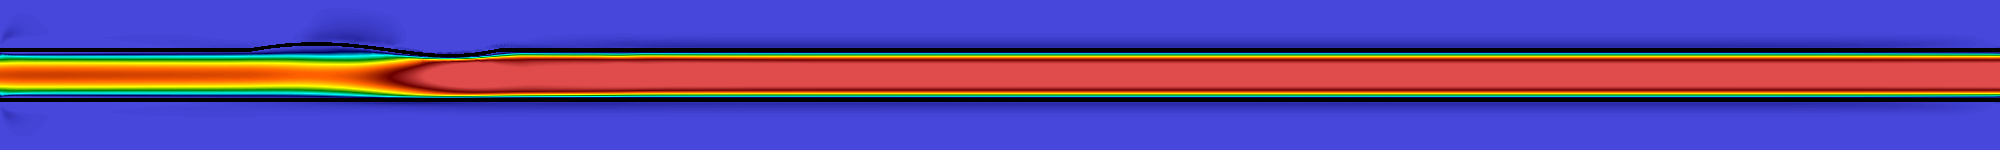
\includegraphics[width=0.98\textwidth]{ch23-ex7-u-t2.png}\\
\scriptsize The whole channel at $t = 2$ s (\code{caseC}, $\mathrm{Re} = 500$): $u$ from $0$ to $10$ cm/s; the two walls in black. The parabola enters at the left; the elastic segment ($5 < x < 10$) is swinging back from an outward bulge, and the fluid it releases runs down the channel faster than the inflow (the red slug).
\footnotesize
\begin{itemize}
  \item The box is $40$ long and $3$ high; the picture is to scale. The fluid above and below the walls is at rest except where the walls move; the channel between them carries the stream. Four grid levels follow the walls, as chapter 22's levels picture showed for the plate.
  \item What happened (from \code{upperoutput.ex2}): as the ramp raised the inflow, the pressure upstream of the segment rose to $87$ dyn/cm$^2$, above $p_e = 49$, and by $t = 1$ the segment had bulged \emph{outward} by $0.59$ cm; by $t = 1.5$ it was at $0.51$, and at $t = 2$ it is an S-shape, $0.12$ out upstream and $0.11$ in downstream. Luo and Pedley's steady collapse needs the channel pressure below $p_e$: a longer run, or \code{caseS2}'s slower stream and softer wall.
\end{itemize}
\sourcecredit{IBAMR 0.19.0, \code{IBFE/explicit/ex7} \code{caseC} to $t = 2$ (\code{/root/work/0.19.0/ibfe\_ex7}); \code{wsl/final/visit\_ch23.sh}.}
\end{frame}

% 24
\begin{frame}{What you should see (2): the elastic segment}
\label{fr:see2}
\centering
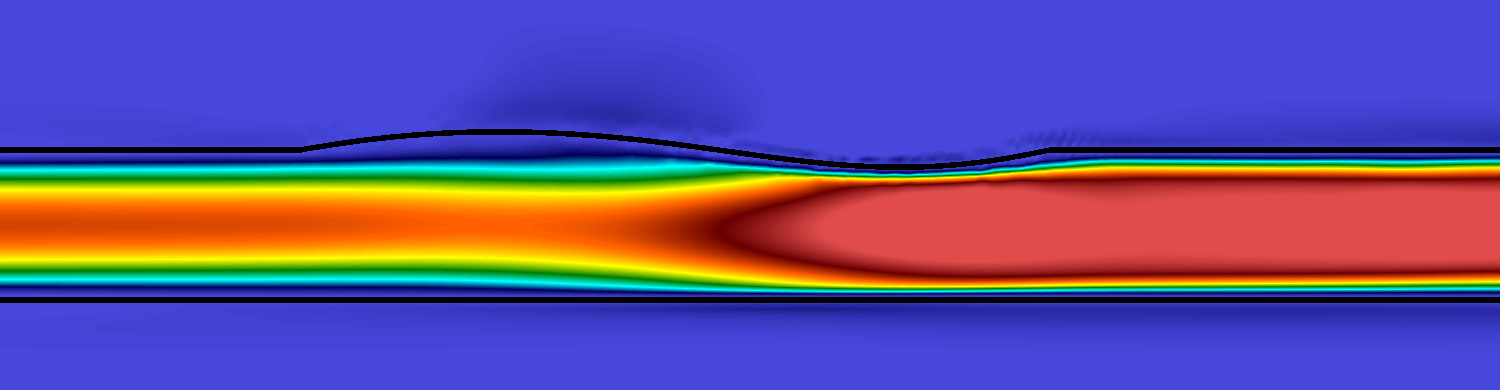
\includegraphics[width=0.62\textwidth]{ch23-ex7-zoom-t2.png}\\
{\tiny $u$ ($0$ to $10$ cm/s) near the segment, $3 < x < 13$, at $t = 2$ s: the wall is out upstream and in downstream, and the stream speeds up where the channel narrows.}\\[1pt]
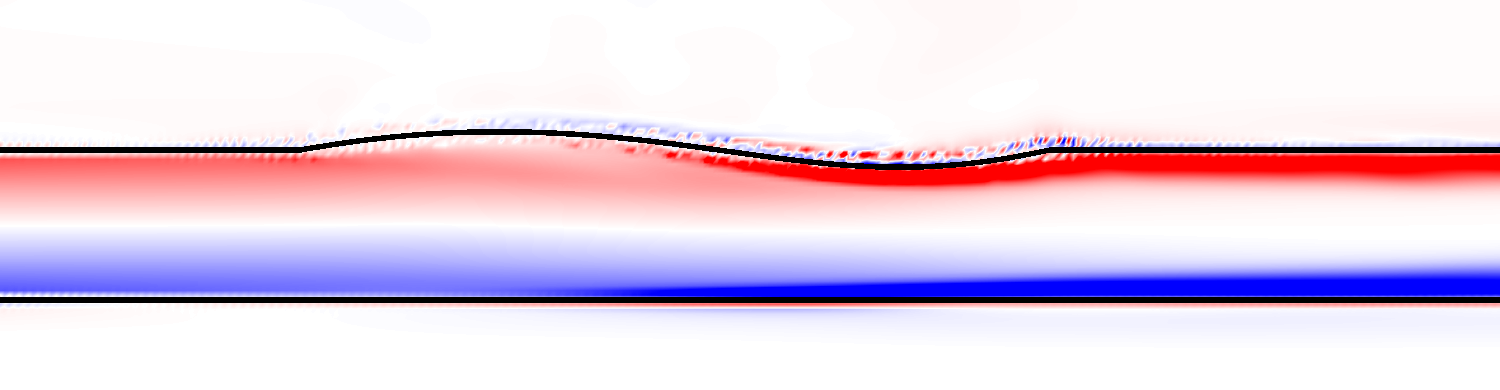
\includegraphics[width=0.62\textwidth]{ch23-ex7-omega-t2.png}\\
{\tiny Vorticity ($\pm50$ s$^{-1}$) in the same window: the boundary layers on both walls (opposite signs), and the speckle of a thin wall that moves through the grid.}
\end{frame}

% 24b
\begin{frame}{What you should see (3): the pressure}
\label{fr:see3}
\centering
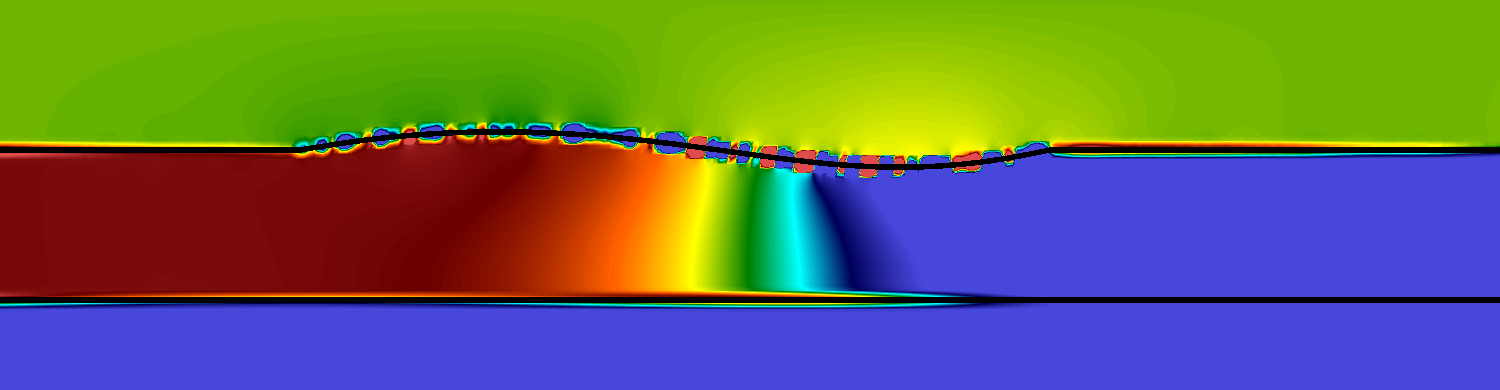
\includegraphics[width=0.62\textwidth]{ch23-ex7-p-t2.png}\\
{\tiny Pressure ($0$ to $100$ dyn/cm$^2$) in the same window at $t = 2$ s.}
\footnotesize
\begin{itemize}
  \item Above the upper wall the pressure is $49$ dyn/cm$^2$, the $p_e$ the top face imposes; below the lower wall it is about $0$, the bottom face's traction. The walls carry the difference.
  \item In the channel the pressure is $87$ upstream of the segment, $62$ at its middle, $-5$ just beyond it and $-10$ at $x = 20$, then back to about $0$ at the free outflow: at this instant almost the whole pressure drop of the channel sits across the segment, because the segment's downstream half is bent in and the released slug is accelerating.
  \item The segment moves toward the lower pressure: out where the channel's $87$ exceeds $p_e$, in where the channel's $-5$ is below it. The speckle along the segment is the pressure jump across a thin wall, which the IB kernel smears over a few cells (chapter 19: \code{use\_jump\_conditions} is the sharper alternative).
\end{itemize}
\end{frame}

% 25
\begin{frame}{Reading any other example with the same map}
\label{fr:recipe}
\footnotesize
\begin{enumerate}
  \item \al{Find \code{ModelData}} (or the functions above \code{main}): what the body is made of and what moves it. Every example's physics is there, in a few dozen lines.
  \item \al{Find every \code{register}:} \code{grep -n register example.cpp}. Each call is one of chapter 19's hooks (stress, body force, surface force, mapping, initial velocity) on one part, or a fluid-side hook (initial conditions, boundary conditions, body force, writers).
  \item \al{Find every \code{getComponentDatabase("...")}:} the list of input blocks the program reads, and so the list of blocks you can change. A block in the input that no call names is dead (slide \ref{fr:sponge2}).
  \item \al{Find \code{build\_} or \code{read(}:} how the mesh comes to be, and which input keys size it.
  \item \al{Find the time loop} and what is in its output block beyond the standard four; and what \code{output\_data} (or \code{postprocess\_data}) writes.
  \item \al{Date the file} by its headers and start-up (slide \ref{fr:legacy}), and update it before you build.
\end{enumerate}
\begin{punchbox}
\footnotesize Chapter 25 applies this to IBAMR's other IBFE examples; chapter 15 did it for the IB ones. The course's own files (chapters 17--22) follow the same map, with \code{main.C} for \code{example.cpp}.
\end{punchbox}
\end{frame}

% 26
\begin{frame}{What can go wrong}
\label{fr:wrong}
\scriptsize
\renewcommand{\arraystretch}{0.95}
\begin{tabular}{@{}L{0.40\textwidth}L{0.52\textwidth}@{}}
\toprule
symptom & cause and fix \\
\midrule
\code{'IBTKInit' was not declared}, or \code{SAMRAI\_MPI::setCommunicator} errors & the 2020 start-up against today's headers, or the reverse; use slide \ref{fr:startup}'s current block (chapter 17) \\
\code{'NULL' was not declared} / \code{AutoPtr} errors & \code{nullptr}, \code{std::unique\_ptr} (slide \ref{fr:legacy}) \\
an input block is ignored & its name differs from the \code{getComponentDatabase} string, or its keys from what the class reads (the sponge layer); check \code{// input used} in the log \\
``Unsupported solver type'' & \code{Main.solver\_type} is not \code{"STAGGERED"} or \code{"COLLOCATED"} \\
a crash at the very end of a run & an object created outside the inner braces, destroyed after the libraries shut down \\
the second part has no stiffness & no stress registered on it: in \code{ex7} that is intended for the lower wall \\
nothing in \code{output\_data}'s folder & \code{data\_dump\_interval = 0} (the default), or the folder name empty \\
``Simulation time'' never advances & the step is tiny: \code{dt\_max}, or a CFL limit from a velocity that blew up \\
\code{error\_on\_dt\_change} abort after a restart & the restarted run's \code{DT} differs from the original's \\
\code{mpirun} refuses to start as root & Open MPI wants \code{--allow-run-as-root} (or the two \code{OMPI\_ALLOW\_RUN\_AS\_ROOT*} variables) in a container or WSL root shell \\
\bottomrule
\end{tabular}
\end{frame}

% 27
\begin{frame}{What the 2020 file had that is now Part X}
\label{fr:legacy}
\footnotesize
\begin{tabular}{@{}L{0.46\textwidth}L{0.46\textwidth}@{}}
\toprule
2020 (\code{ex7} as the lecture showed it) & 0.19.0 \\
\midrule
\code{\#include <IBAMR\_config.h>}, \code{<IBTK\_config.h>} & gone; \code{<ibtk/IBTKInit.h>}, \code{<ibtk/IBTK\_MPI.h>} added \\
\code{LibMeshInit init(argc, argv); SAMRAI\_MPI::setCommunicator(...); SAMRAIManager::startup();} \ldots \code{shutdown()} & \code{IBTKInit ibtk\_init(argc, argv, MPI\_COMM\_WORLD); const LibMeshInit\& init = ibtk\_init.getLibMeshInit();} \\
\code{static\_cast<RobinBcCoefStrategy}\newline\code{<NDIM>*>(NULL)} & \code{nullptr} \\
\code{std::unique\_ptr<ExodusII\_IO> io(uses\_exodus ? new ExodusII\_IO(mesh) : NULL)} & \code{uses\_exodus ? std::make\_unique<ExodusII\_IO>(mesh) : nullptr} \\
\code{MathUtilities<double>::equalEps(loop\_time, loop\_time\_end)} & \code{IBTK::rel\_equal\_eps(loop\_time, loop\_time\_end)} \\
\code{SAMRAI\_MPI::getRank()} in \code{output\_data} & \code{IBTK\_MPI::getRank()} \\
the lecture's C++ primer from tutorialspoint and the stack from IBAMR's README & slides \ref{fr:stack}--\ref{fr:cpp2}, in this series' words \\
``not totally sure what sponge layer does'' & slide \ref{fr:sponge2} \\
\bottomrule
\end{tabular}
\end{frame}

% 28
\begin{frame}{Exercises}
\label{fr:exercises}
\footnotesize
\begin{enumerate}
  \item Rename the sponge layer's keys to \code{forcing\_enabled\_0}, \code{forcing\_enabled\_1} and run \code{caseC} to $0.5$ s with and without: compare $v$ in the first cell at the inflow (a VisIt lineout, chapter 29).
  \item Add a chapter 22 force integral to \code{output\_data} for the upper wall's tether, set \code{data\_dump\_interval}, and plot the force the fluid puts on the rigid parts of the wall against time.
  \item Give the lower wall the same stress function as the upper one with its own elastic segment, and watch the channel collapse from both sides.
  \item Run \code{caseS2} to $5$ s (a few hours): does the segment begin to oscillate?
  \item Replace the walls by a mesh read from a file (chapter 18) with the same geometry, and check that the run is the same.
  \item Take the course's \code{main.C} of chapter 17 and mark its seventeen blocks with the map of slides \ref{fr:map}--\ref{fr:map2}; which are missing, and which are extra?
\end{enumerate}
\end{frame}

% 29
\begin{frame}{Rules of thumb}
\label{fr:thumb}
\small
\begin{itemize}
  \item Every IBAMR main file is the same seventeen blocks in the same order; learn the map once.
  \item The physics is in \code{ModelData} and the \code{register} calls; everything else is plumbing you copy.
  \item An input block is read only if a \code{getComponentDatabase} names it, and a key only if the class spells it the same way; the log's \code{// input used} tells you.
  \item Objects live inside the inner braces; \code{IBTKInit} outside.
  \item \code{output\_data} is yours: a measurement or a state dump, with the signature kept.
  \item Date a file by its headers; update the start-up, \code{nullptr} and \code{unique\_ptr} before you build.
\end{itemize}
\end{frame}

% 30
\begin{frame}{Summary}
\label{fr:summary}
\footnotesize
\begin{enumerate}
  \item \code{ex7} is a collapsible channel: two thin tethered walls built in the program, an elastic St.\ Venant--Kirchhoff segment in the upper one, a ramped parabolic inflow, a free outflow, and an external pressure applied on the top face of the box; three cases at $\mathrm{Re} = 500$, $200$ and $77$.
  \item The file is seventeen blocks: headers, model callbacks, start-up (\code{IBTKInit}), \code{AppInitializer} and the \code{Main} keys with their aliases, meshes, solvers, the six grid objects, the IBFE registrations per part, initial and boundary conditions from muParser, a body force, writers, initialization, the time loop with its four output \code{if}s, and \code{output\_data}.
  \item The sponge layer damps a velocity component near a face; in \code{ex7} its keys are misspelt and it is off.
  \item Run to $2$ s on four cores in an hour: the ramp raises the upstream pressure above $p_e$, the segment bulges outward by $0.6$ cm, then swings back and pumps a slug of fluid down the channel.
  \item The 2020 version differs in the start-up, \code{NULL}, \code{unique\_ptr} and the time test; the map, and the recipe for reading any other example, are the same.
\end{enumerate}
\begin{homebox}
\footnotesize Chapter 24: IBFE with advection--diffusion, a concentration carried by the flow past a moving body.
\end{homebox}
\end{frame}

% 31
\begin{frame}{Recordings (listed, not incorporated)}
\label{fr:videos}
\small The 2020 Zoom recording of \emph{Lecture 8-IBFE-Going through a main file} is listed in the front matter's video list (chapter 0.1). The lecture's nine code screenshots are transcribed on slides \ref{fr:headers}--\ref{fr:outblock} from the 0.19.0 file, with the 2020 differences on slide \ref{fr:legacy}.
\end{frame}

% 32
\begin{frame}{References and credits}
\label{fr:refs}
\scriptsize
\begin{itemize}
  \item IBAMR 0.19.0: \code{examples/IBFE/explicit/ex7/example.cpp} and its three inputs; \code{ibtk/src/utilities/AppInitializer.cpp}, \code{IBTKInit.cpp}; \code{src/navier\_stokes/SpongeLayerForceFunction.cpp}; \code{include/ibamr/app\_namespaces.h}. \url{https://github.com/IBAMR/IBAMR}; documentation \url{https://ibamr.github.io/docs}.
  \item The course material: \emph{Lecture 8-IBFE-Going through a main file} (2020; its code screenshots and notes).
  \item libMesh: \code{MeshTools::Generation::build\_square}, \url{https://libmesh.github.io}. SAMRAI, PETSc, hypre, muParser, HDF5: the libraries of slides \ref{fr:stack}--\ref{fr:stack2}.
  \item X. Y. Luo and T. J. Pedley, \emph{A numerical simulation of unsteady flow in a two-dimensional collapsible channel}, J.\ Fluid Mech.\ 314 (1996) 191--225: the geometry and the external-pressure set-up that \code{ex7} follows.
  \item The run: \code{/root/work/0.19.0/ibfe\_ex7} (IBAMR 0.19.0, four cores); figures with VisIt 3.5, \code{wsl/final/visit\_ch23.sh}.
\end{itemize}
\end{frame}

\end{document}
